\documentclass[a4paper, UTF8, 12pt]{ctexart}
\usepackage{geometry}
\usepackage{listings}
\usepackage{xcolor}
\usepackage{amsmath}
\usepackage{graphicx}
\usepackage{arydshln}
\geometry{left=1.5cm, right=1.5cm, top=1.5cm, bottom=2.5cm}
\allowdisplaybreaks

\title{模式识别与机器学习作业--第三章}
\author{2019.9.22}
\date{}
\begin{document}
    \maketitle
    \pagestyle{plain}
    \allowdisplaybreaks

    % \subsection*{作业1}
    \textbf{1. 在一个10类的模式识别问题中,有3类单独满足多类情况1,其余的类别满足多类情况2。问该模式识别问题所需判别函数的最少数目是多少?} 

    答:由题意,首先由于该模式种有三类单独满足多类情况1,所以可以先把这一部分看成是4分类问题,
    此处需要4个判别函数;之后剩下的七个模式类别可以看作第四类中再进行二次划分的情况,
    这里需要M(m-1)/2=21中判别函数。所以整个问题一共最少需要判别函数为21+4=25个。 \\

    % \subsection*{作业2}
    \textbf{2. 一个三类问题,其判别函数为: \ \ {d1(x)=-x1, d2(x)=x1+x2-1, d3(x)=x1-x2-1} }
    
    1). 设这些函数是在多类情况1条件下确定的,绘出其判别界面和每一个模式类别的区域。 
    
    2). 设为多类情况2,并使:d12(x)= d1(x), d13(x)= d2(x), d23(x)= d3(x)。
    绘出其判别界面和多类情况2的区域。 
    
    3). 设d1(x), d2(x)和d3(x)是在多类情况3的条件下确定的,绘出其判别界面和每类的区域。 \\

    \centerline{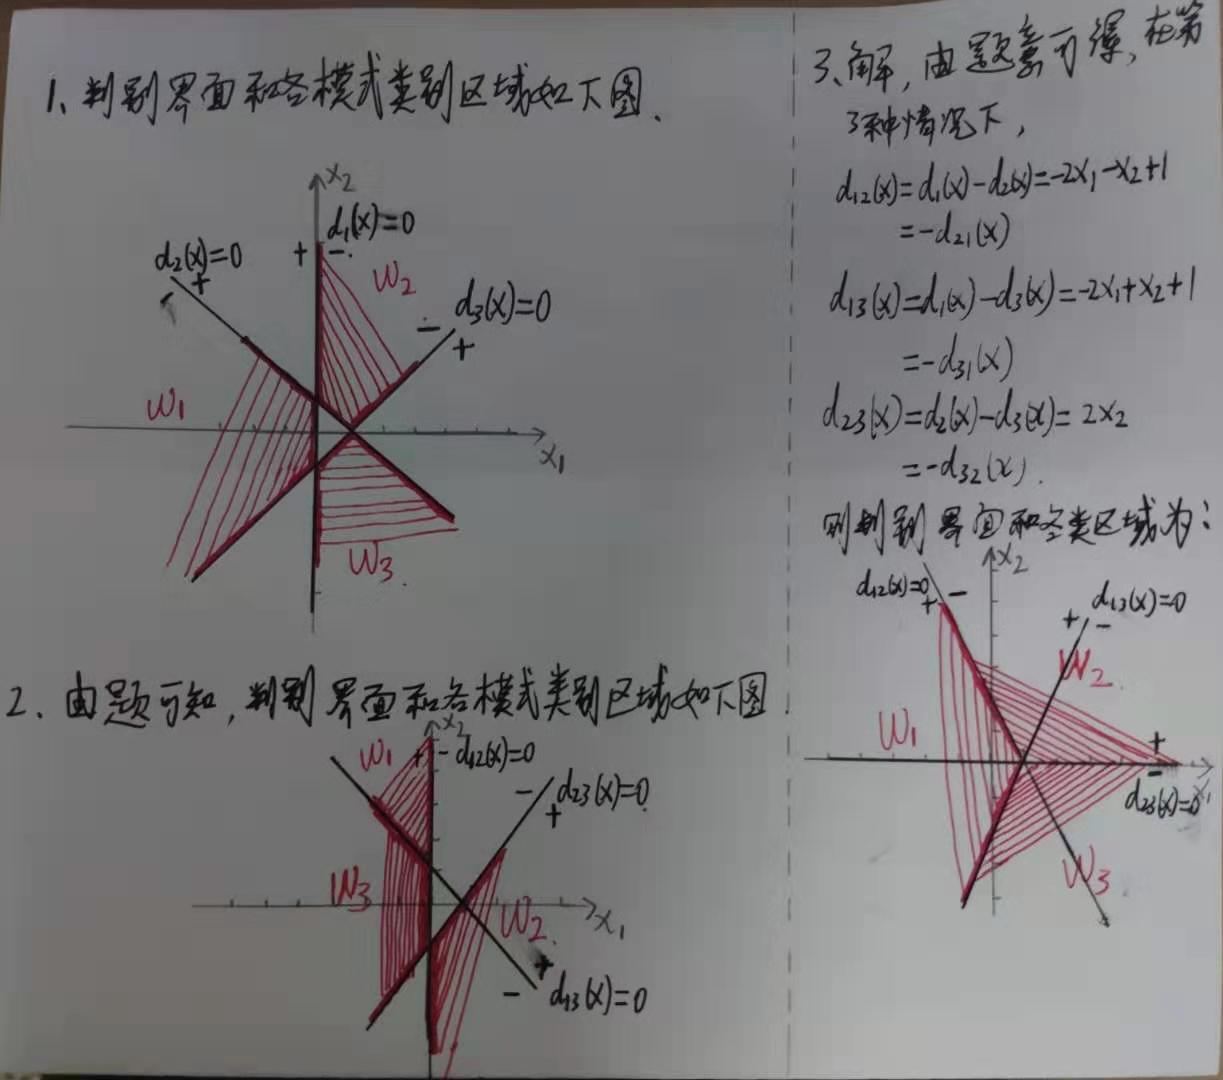
\includegraphics[ scale=0.33]{asw2.jpg}}

    % \subsection*{作业3}
    \newpage
    \textbf{3. 两类模式,每类包括5个3维不同的模式,且良好分布。如果它们是线性可分的,
    问权向量至少需要几个系数分量?假如要建立二次的多项式判别函数,又至少需要几个系数分量?
    (设模式的良好分布不因模式变化而改变。)}

    答:由题意,当两类模式线性可分且每类模式为3维时,权向量的分量
    至少为 $(n+1)=4$个;当需要建立二次多项式判别函数时,此时需
    要的系数分量至少为$\frac{(n+1)(n+2)}{2}=(4\times 5)/2=10.$ \\
    
    % \subsection*{作业4}
    \textbf{4. (1)用感知器算法求下列模式分类的解向量w:}
    \begin{equation*}
        \begin{split}
            w_1 &: \ \left\{ {\left(0, 0, 0 \right)}^T, {\left(1, 0, 0\right)}^T, {\left(1, 0, 1\right)}^T,{\left(1, 1, 0\right)}^T \right\}   \\
            w_2 &: \ \left\{{\left(0, 0, 1\right)}^T, {\left(0, 1, 1\right)}^T, {\left(0, 1, 0\right)}^T, {\left(1, 1, 1\right)}^T \right\}
        \end{split}
    \end{equation*} 

    答:首先将$w_2$类的样本乘(-1),并写成增广向量形式,得到新的样本如下
    \begin{equation*}
        \begin{split}
            w_1 &: \ \left\{ {\left(0, 0, 0, 1 \right)}^T, {\left(1, 0, 0, 1\right)}^T, {\left(1, 0, 1, 1\right)}^T,{\left(1, 1, 0, 1\right)}^T \right\}   \\
            w_2 &: \ \left\{{\left(0, 0, -1, -1\right)}^T, {\left(0, -1, -1, -1\right)}^T, {\left(0, -1, 0, -1\right)}^T, {\left(-1, -1, -1, -1\right)}^T \right\}
        \end{split}
    \end{equation*} 

    取$C=1,\ \  w(1) = (0,0,0,0)^T$,则迭代过程如下:
    % \begin{equation*}
        \begin{align*}
            epi&sode1: \\
            &w^T(1)x_1 = (0,0,0,0)(0,0,0,1)^T=0 \not> 0, &&w(2)=w(1)+x_1=(0,0,0,1)^T \\
            &w^T(2)x_2 = (0,0,0,1)(1,0,0,1)^T=1 > 0, &&w(3)=w(2)=(0,0,0,1)^T \\
            &w^T(3)x_3 = (0,0,0,1)(1,0,1,1)^T=1 > 0, &&w(4)=w(3)=(0,0,0,1)^T \\
            &w^T(4)x_4 = (0,0,0,1)(1,1,0,1)^T=1 > 0, &&w(5)=w(4)=(0,0,0,1)^T \\ 
            &w^T(5)x_5 = (0,0,0,1)(0,0,-1,-1)^T=-1 \not> 0, &&w(6)=w(5)+x_5=(0,0,-1,0)^T \\
            &w^T(6)x_6 = (0,0,-1,0)(0,-1,-1,-1)^T=1 > 0, &&w(7)=w(6)=(0,0,-1,0)^T \\
            &w^T(7)x_7 = (0,0,-1,0)(0,-1,0,-1)^T=0 \not> 0, &&w(8)=w(7)+x_7=(0,-1,-1,-1)^T \\
            &w^T(8)x_8 = (0,-1,-1,-1)(-1,-1,-1,-1)^T=3 > 0, &&w(9)=w(8)=(0,-1,-1,-1)^T \\
            epi&sode2: \\
            &w^T(9)x_1 = (0,-1,-1,-1)(0,0,0,1)^T=-1 \not> 0, &&w(10)=w(9)+x_1=(0,-1,-1,0)^T \\
            &w^T(10)x_2 = (0,-1,-1,0)(1,0,0,1)^T=0 \not> 0, &&w(11)=w(10)+x_2=(1,-1,-1,1)^T \\
            &w^T(11)x_3 = (1,-1,-1,1)(1,0,1,1)^T=1 > 0, &&w(12)=w(11)=(1,-1,-1,1)^T \\
            &w^T(12)x_4 = (1,-1,-1,1)(1,1,0,1)^T=1 > 0, &&w(13)=w(12)=(1,-1,-1,1)^T \\ 
            &w^T(13)x_5 = (1,-1,-1,1)(0,0,-1,-1)^T=0 \not> 0, &&w(14)=w(13)+x_5=(1,-1,-2,0)^T \\
            &w^T(14)x_6 = (1,-1,-2,0)(0,-1,-1,-1)^T=3 > 0, &&w(15)=w(14)=(1,-1,-2,0)^T \\
            &w^T(15)x_7 = (1,-1,-2,0)(0,-1,0,-1)^T=1 > 0, &&w(16)=w(15)=(1,-1,-2,0)^T \\
            &w^T(16)x_8 = (1,-1,-2,0)(-1,-1,-1,-1)^T=2 > 0, &&w(17)=w(16)+x_8=(1,-1,-2,0)^T \\
            epi&sode3: \\
            &w^T(17)x_1 = (1,-1,-2,0)(0,0,0,1)^T=0 \not> 0, &&w(18)=w(17)+x_1=(1,-1,-2,1)^T \\
            &w^T(18)x_2 = (1,-1,-2,1)(1,0,0,1)^T=2 > 0, &&w(19)=w(18)=(1,-1,-2,1)^T \\
            &w^T(19)x_3 = (1,-1,-2,1)(1,0,1,1)^T=0 \not> 0, &&w(20)=w(19)+x_3=(2,-1,-1,2)^T \\
            &w^T(20)x_4 = (2,-1,-1,2)(1,1,0,1)^T=3 \not> 0, &&w(21)=w(20)=(2,-1,-1,2)^T \\ 
            &w^T(21)x_5 = (2,-1,-1,2)(0,0,-1,-1)^T=-1 \not> 0, &&w(22)=w(21)+x_5=(2,-1,-2,1)^T \\
            &w^T(22)x_6 = (2,-1,-2,1)(0,-1,-1,-1)^T=2 > 0, &&w(23)=w(22)=(2,-1,-2,1)^T \\
            &w^T(23)x_7 = (2,-1,-2,1)(0,-1,0,-1)^T=0 \not> 0, &&w(24)=w(23)+x_7=(2,-2,-2,0)^T \\
            &w^T(24)x_8 = (2,-2,-2,0)(-1,-1,-1,-1)^T=2 > 0, &&w(25)=w(24)+x_8=(2,-2,-2,0)^T \\
            epi&sode4: \\
            &w^T(25)x_1 = (2,-2,-2,0)(0,0,0,1)^T=0 \not> 0, &&w(26)=w(25)+x_1=(2,-2,-2,1)^T \\
            &w^T(26)x_2 = (2,-2,-2,1)(1,0,0,1)^T=3 > 0, &&w(27)=w(26)=(2,-2,-2,1)^T \\
            &w^T(27)x_3 = (2,-2,-2,1)(1,0,1,1)^T=1 > 0, &&w(28)=w(27)=(2,-2,-2,1)^T \\
            &w^T(28)x_4 = (2,-2,-2,1)(1,1,0,1)^T=1 > 0, &&w(29)=w(28)=(2,-2,-2,1)^T \\ 
            &w^T(29)x_5 = (2,-2,-2,1)(0,0,-1,-1)^T=1 > 0, &&w(30)=w(29)=(2,-2,-2,1)^T \\
            &w^T(30)x_6 = (2,-2,-2,1)(0,-1,-1,-1)^T=3 > 0, &&w(31)=w(30)=(2,-2,-2,1)^T \\
            &w^T(31)x_7 = (2,-2,-2,1)(0,-1,0,-1)^T=1 > 0, &&w(32)=w(31)=(2,-2,-2,1)^T \\
            &w^T(32)x_8 = (2,-2,-2,1)(-1,-1,-1,-1)^T=1 > 0, &&w(33)=w(32)=(2,-2,-2,1)^T \\
            epi&sode5: \\
            &w^T(33)x_1 = (2,-2,-2,1)(0,0,0,1)^T=1 > 0, &&w(34)=w(33)=(2,-2,-2,1)^T \\
            &w^T(34)x_2 = (2,-2,-2,1)(1,0,0,1)^T=3 > 0, &&w(35)=w(34)=(2,-2,-2,1)^T \\
            &w^T(35)x_3 = (2,-2,-2,1)(1,0,1,1)^T=1 > 0, &&w(36)=w(35)=(2,-2,-2,1)^T \\
            &w^T(36)x_4 = (2,-2,-2,1)(1,1,0,1)^T=1 > 0, &&w(37)=w(36)=(2,-2,-2,1)^T \\ 
            &w^T(37)x_5 = (2,-2,-2,1)(0,0,-1,-1)^T=1 > 0, &&w(38)=w(37)=(2,-2,-2,1)^T \\
            &w^T(38)x_6 = (2,-2,-2,1)(0,-1,-1,-1)^T=3 > 0, &&w(39)=w(38)=(2,-2,-2,1)^T \\
            &w^T(39)x_7 = (2,-2,-2,1)(0,-1,0,-1)^T=1 > 0, &&w(40)=w(39)=(2,-2,-2,1)^T \\
            &w^T(40)x_8 = (2,-2,-2,1)(-1,-1,-1,-1)^T=1 > 0, &&w(41)=w(40)=(2,-2,-2,1)^T 
        \end{align*}
        
        所以最终的解向量为$w=(2,-2,-2,1)^T$,
        相应的判别函数为$d(x)=2x_1-2x_2-2x_3+1$ \\
    % \end{equation*}

    % \textbf{(2). 编写求解上述问题的感知器算法程序。}

    % 程序及运行结果如下 \\


    % \subsection*{作业5}
    \textbf{5. 用多类感知器算法求下列模式的判别函数:}
    \begin{equation*}
        \begin{split}
            w_1  &: \ {\left(-1,-1\right)}^T \\
            w_2  &: \ {\left(0,0\right)}^T \\
            w_3  &: \ {\left(1,1\right)}^T
        \end{split}
    \end{equation*}

    答:首先将模式样本写成增广向量形式,得到新的样本如下
    \begin{equation*}
            x_1 = {\left(-1,-1,1\right)}^T ,\ \ 
            x_2 = {\left(0,0,1\right)}^T ,\ \  
            x_3 = {\left(1,1,1\right)}^T
    \end{equation*}

    取$C=1,\  w_1(1) = w_2(1) = w_3(1) = (0,0,0)^T$,则迭代过程如下:
    % \begin{equation*}
        \begin{align*}
          episode1: &k=1,x_1 = {\left(-1,-1,1\right)}^T ,\\
            &d_1(1)=w_1^T(1)x_1=(0,0,0)(-1,-1,1)^T=0 \\
            &d_2(1)=w_2^T(1)x_1=(0,0,0)(-1,-1,1)^T=0 \\
            &d_3(1)=w_3^T(1)x_1=(0,0,0)(-1,-1,1)^T=0 \\
            & d_1(1) \not> d_2(1) ,\ \  d_1(1) \not> d_3(1) \\
            &w_1(2)=w_1(1)+x_1=(0,0,0)^T+(-1,-1,1)^T=(-1,-1,1)^T \\
            &w_2(2)=w_2(1)-x_1=(0,0,0)^T-(-1,-1,1)^T=(1,1,-1)^T \\
            &w_3(2)=w_3(1)-x_1=(0,0,0)^T-(-1,-1,1)^T=(1,1,-1)^T \\
          episode2: &k=2,x_2 = {\left(0,0,1\right)}^T ,\\
            &d_1(2)=w_1^T(2)x_2=(-1,-1,1)(0,0,1)^T=1 \\
            &d_2(2)=w_2^T(2)x_2=(1,1,-1)(0,0,1)^T=-1 \\
            &d_3(2)=w_3^T(2)x_2=(1,1,-1)(0,0,1)^T=-1 \\
            & d_2(2) \not> d_1(2) ,\ \  d_2(2) \not> d_3(2) \\
            &w_1(3)=w_1(2)-x_2=(-1,-1,1)^T-(0,0,1)^T=(-1,-1,0)^T \\
            &w_2(3)=w_2(2)+x_2=(1,1,-1)^T+(0,0,1)^T=(1,1,0)^T \\
            &w_3(3)=w_3(2)-x_2=(1,1,-1)^T-(0,0,1)^T=(1,1,-2)^T \\
          episode3 : &k=3,x_3= {\left(1,1,1 \right)}^T ,\\
            &d_1(3)=w_1^T(3)x_3=(-1,-1,0)(1,1,1)^T= -2\\
            &d_2(3)=w_2^T(3)x_3=(1,1,0)(1,1,1)^T= 2 \\
            &d_3(3)=w_3^T(3)x_3=(1,1,-2)(1,1,1)^T= 0 \\
            & d_3(3) > d_1(3) ,\ \  d_3(3) \not> d_2(3) \\
            &w_1(4)=w_1(3)=(-1,-1,0)^T \\
            &w_2(4)=w_2(3)-x_3=(1,1,0)^T-(1,1,1)^T=(0,0,-1)^T \\
            &w_3(4)=w_3(3)+x_3=(1,1,-2)^T+(1,1,1)^T= (2,2,-1)^T \\
          episode4: &k=4,x_1 = {\left(-1,-1,1\right)}^T ,\\
            &d_1(4)=w_1^T(4)x_1=(-1,-1,0)(-1,-1,1)^T=2 \\
            &d_2(4)=w_2^T(4)x_1=(0,0,-1)(-1,-1,1)^T=-1 \\
            &d_3(4)=w_3^T(4)x_1=(2,2,-1)(-1,-1,1)^T=-5 \\
            & d_1(4) > d_2(4) ,\ \  d_1(4) > d_3(4) \\
            &w_1(5)=w_1(4)=(0,0,1)^T \\
            &w_2(5)=w_2(4)=(0,0,-1)^T \\
            &w_3(5)=w_3(4)=(2,2,-1)^T \\
          episode5: &k=5,x_2 = {\left(0,0,1\right)}^T ,\\
            &d_1(5)=w_1^T(5)x_2=(-1,-1,0)(0,0,1)^T=0 \\
            &d_2(5)=w_2^T(5)x_2=(0,0,-1)(0,0,1)^T=-1 \\
            &d_3(5)=w_3^T(5)x_2=(2,2,-1)(0,0,1)^T=-1 \\
            & d_2(5) \not> d_1(5) ,\ \  d_2(5) \not> d_3(5) \\
            &w_1(6)=w_1(5)-x_2=(-1,-1,0)^T-(0,0,1)^T=(-1,-1,-1)^T \\
            &w_2(6)=w_2(5)+x_2=(0,0,-1)^T+(0,0,1)^T=(0,0,0)^T \\
            &w_3(6)=w_3(5)-x_2=(2,2,-1)^T-(0,0,1)^T=(2,2,-2)^T \\
          episode6 : &k=6,x_3= {\left(1,1,1 \right)}^T ,\\
            &d_1(6)=w_1^T(6)x_3=(-1,-1,-1)(1,1,1)^T= -3\\
            &d_2(6)=w_2^T(6)x_3=(0,0,0)(1,1,1)^T= 0 \\
            &d_3(6)=w_3^T(6)x_3=(2,2,-2)(1,1,1)^T= 2 \\
            & d_3(6) > d_1(6) ,\ \  d_3(3) > d_2(3) \\
            &w_1(7)=w_1(6)=(-1,-1,-1)^T \\
            &w_2(7)=w_2(6)=(0,0,0)^T \\
            &w_3(7)=w_3(6)=(2,2,-2)^T\\
          episode7: &k=7,x_1 = {\left(-1,-1,1\right)}^T ,\\
            &d_1(7)=w_1^T(7)x_1=(-1,-1,-1)(-1,-1,1)^T=1 \\
            &d_2(7)=w_2^T(7)x_1=(0,0,0)(-1,-1,1)^T=0 \\
            &d_3(7)=w_3^T(7)x_1=(2,2,-2)(-1,-1,1)^T=-6 \\
            & d_1(7) > d_2(7) ,\ \  d_1(7) > d_3(7) \\
            &w_1(8)=w_1(7)=(-1,-1,-1)^T \\
            &w_2(8)=w_2(7)=(0,0,0)^T \\
            &w_3(8)=w_3(7)=(2,2,-2)^T \\
          episode8: &k=7,x_2 = {\left(0,0,1\right)}^T ,\\
            &d_1(8)=w_1^T(8)x_2=(-1,-1,-1)(0,0,1)^T=-1 \\
            &d_2(8)=w_2^T(8)x_2=(0,0,0)(0,0,1)^T=0 \\
            &d_3(8)=w_3^T(8)x_2=(2,2,-2)(0,0,1)^T=-2 \\
            & d_2(8) > d_1(8) ,\ \  d_2(5) > d_3(5) \\
            &w_1(9)=w_1(8)-x_2=(-1,-1,-1)^T \\
            &w_2(9)=w_2(8)+x_2=(0,0,0)^T \\
            &w_3(9)=w_3(8)-x_2=(2,2,-2)^T \\
        \end{align*}

        因此,权向量的解为
        \begin{equation*}
            w_1=\left(
                \begin{aligned}
                & -1 \\ &-1 \\ &-1
                \end{aligned} 
            \right) , \ \  
            w_2=\left(
                \begin{aligned}
                    & 0 \\ &0 \\ &0
                \end{aligned} 
            \right), \ \  
            w_3=\left(
                \begin{aligned}
                    & 2 \\ &2 \\ &-2
                \end{aligned} 
            \right)
        \end{equation*}

        相应的判别函数为
        $$\left\{
                \begin{aligned}
                    &d_1 = -x_1-x_2-1 \\
                    &d_2 = 0 \\ 
                    &d_3 = 2x_1+2x_2-2
                \end{aligned} 
            \right.
        $$ \\

    % \subsection*{作业6}
    \textbf{6. 采用梯度法和如下准测函数,式中实数b>0,试导出两类模式的分类算法。} \\
    \centerline{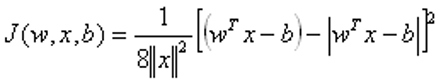
\includegraphics[scale=0.5]{ass6.png}} \\

    答:由题意可知,对准则函数$J$进行微分,得:
    \begin{align*}
        &\frac{\partial{J}}{\partial{w}}=\frac{1}{4\parallel x\parallel^2}\left[
            \left(w^Tx-b\right)-|w^Tx-b|
            \right]\times\left[
            x-x\times sign\right(w^Tx-b)] \\
        &where, \ \ 
        sign(w^T-b)=\left\{
            \begin{aligned}
                1, && w^Tx-b > 0 \\ 
                -1, && w^Tx-b \leq 0
            \end{aligned}
        \right.
    \end{align*}

    由此得到迭代式并化简后得:
    \begin{align*}
        &w(k+1)=w(k)+\frac{C}{4\parallel x\parallel^2}\left[
            \left(w^T(k)x-b\right)-|w^T(k)x-b|
            \right]\times\left[
            x-x\times sign\right(w^T(k)x-b)] \\
        &==>, \\
        &w(k+1)=w(k)+C\left\{
            \begin{aligned}
                &0, && w^T(k)x-b > 0 \\ 
                &\frac{(b-w^T(k)x)}{\parallel x\parallel^2}x, && w^T(k)x-b \leq 0
            \end{aligned}
        \right.
    \end{align*} \\

    % \subsection*{作业7}
    \newpage
    \textbf{7. 用二次埃尔米特多项式的势函数算法求解以下模式的分类问题} \newline
    \begin{equation*}
        \begin{split}
            w_1: \ \left\{ {\left(0,1 \right)}^T, {\left(0,-1\right)}^T \right\}, \ \ \ 
            w_2: \ \left\{{\left(1,0\right)}^T, {\left(-1,0\right)}^T \right\}
        \end{split}
    \end{equation*}
    % 解题过程如下图所示:\\
    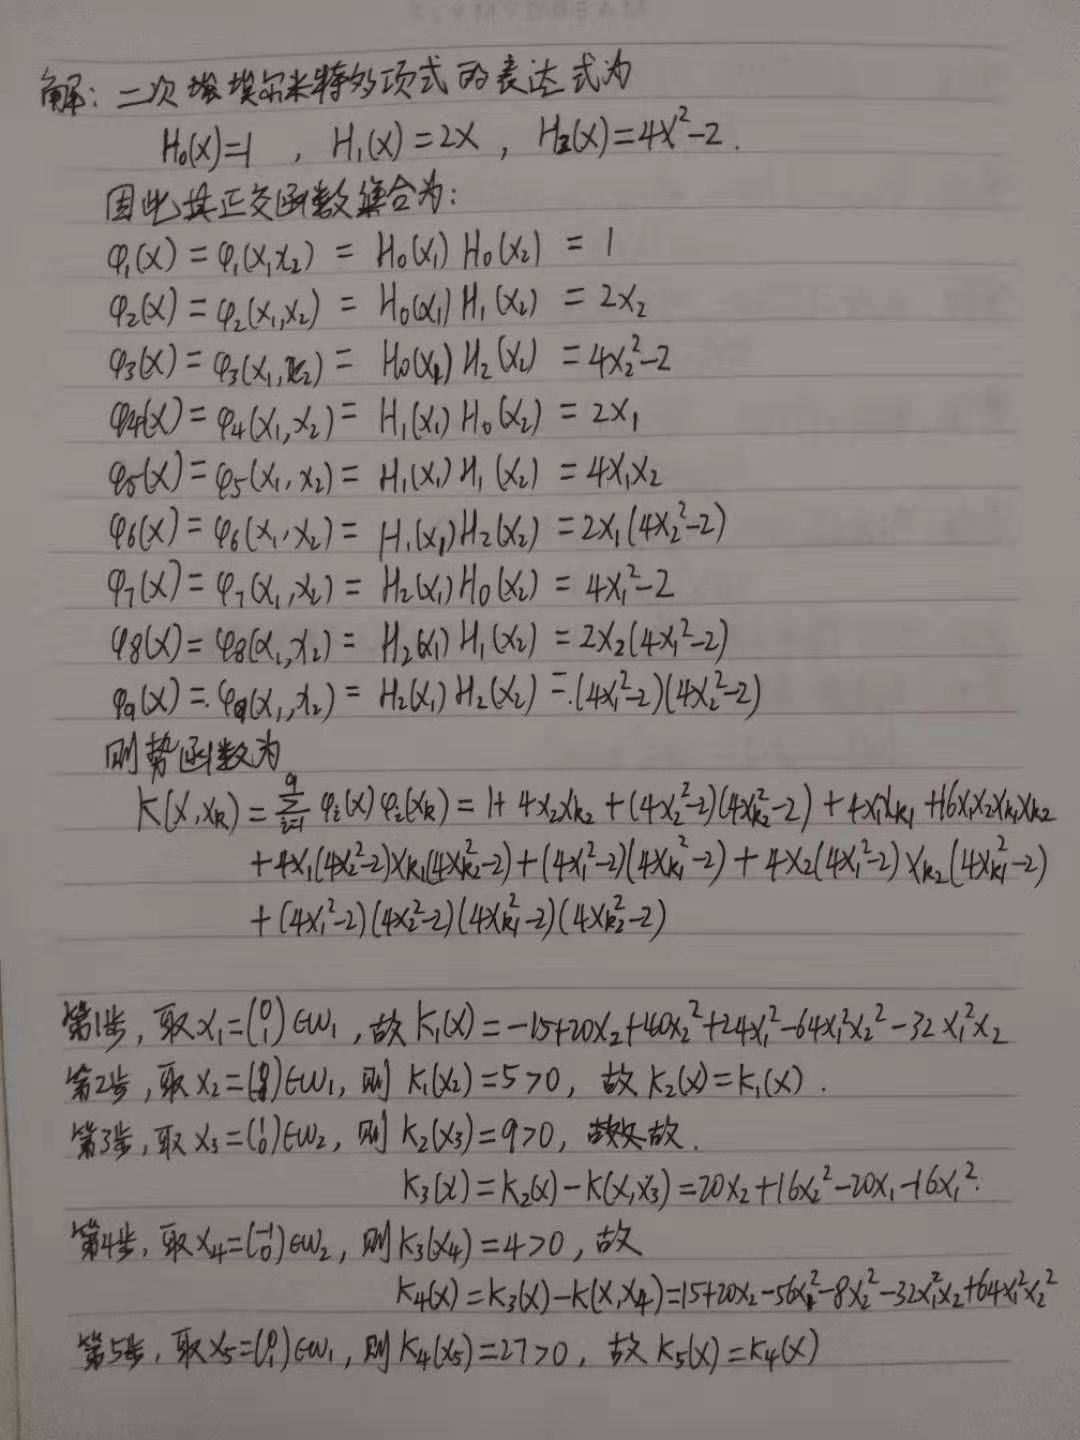
\includegraphics[scale=0.46]{asw7_0.jpg}

    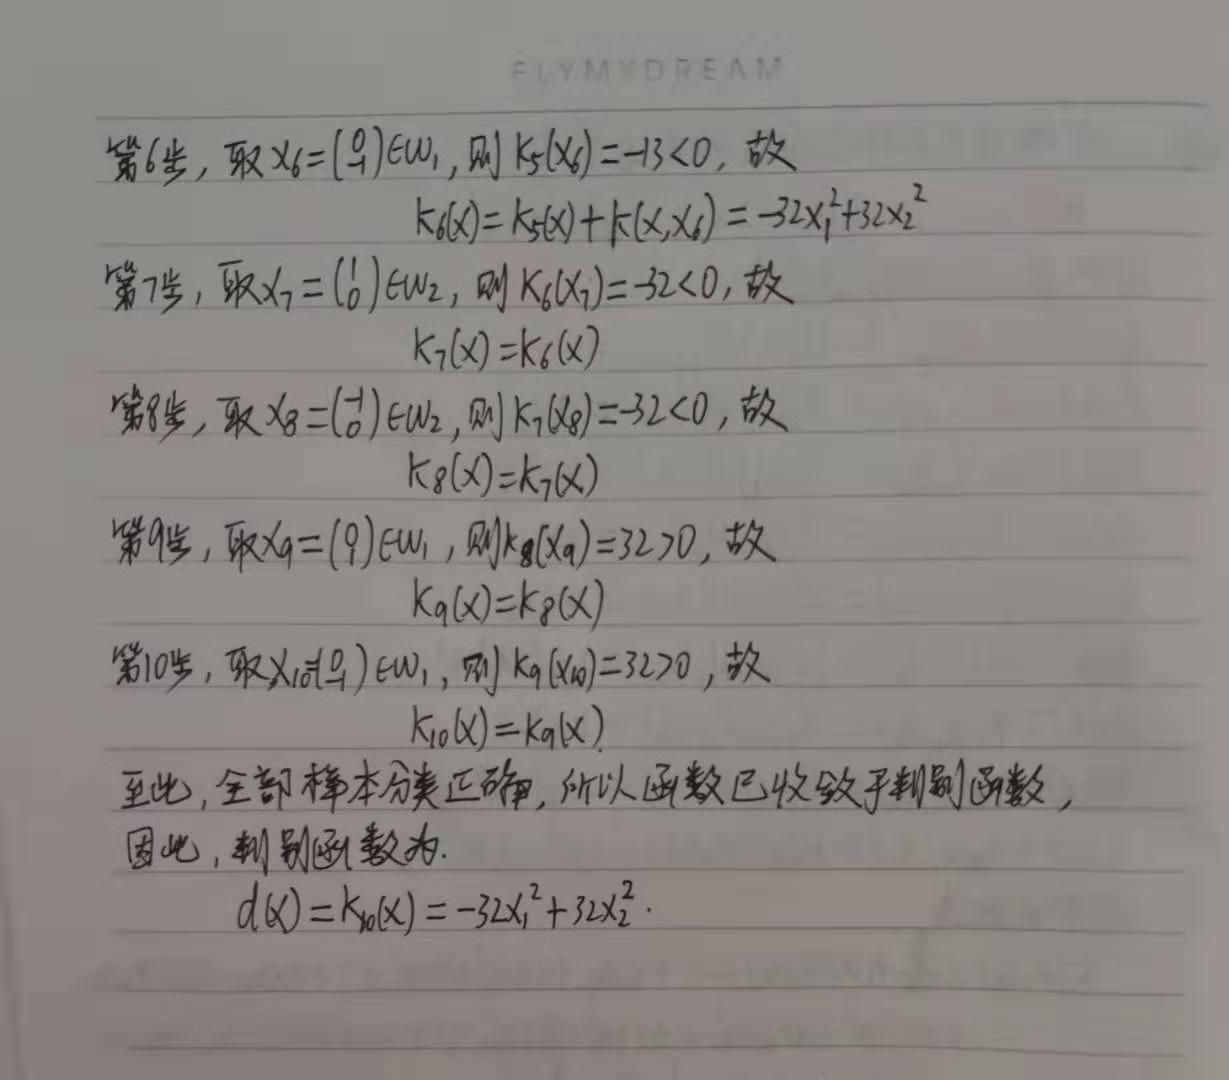
\includegraphics[scale=0.4]{asw7_1.jpg} \\ \\

    % \subsection*{作业8}
    \newpage
    \textbf{8. 用下列势函数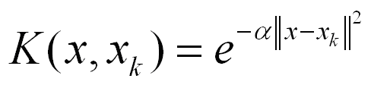
\includegraphics[scale=0.5]{ass8.png}求解以下模式分类问题:}
    \begin{equation*}
        \begin{split}
            w_1: \ \left\{ {\left(0,1 \right)}^T, {\left(0,-1\right)}^T \right\}, \ \ 
            w_2: \ \left\{{\left(1,0\right)}^T, {\left(-1,0\right)}^T \right\}
        \end{split}
    \end{equation*}
    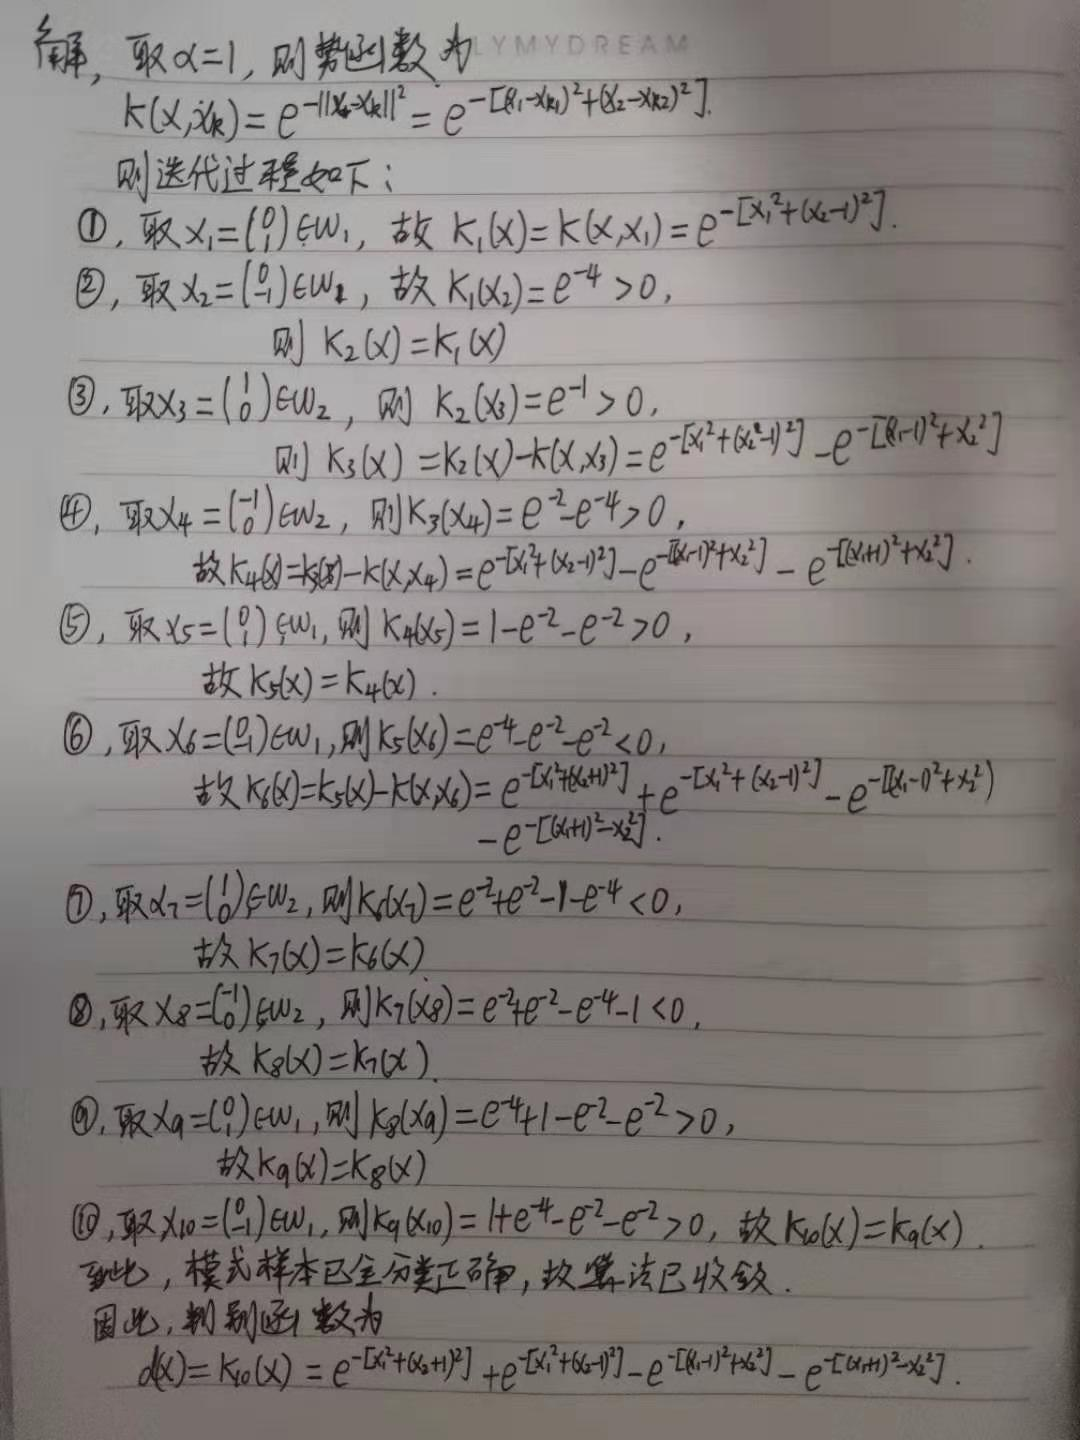
\includegraphics[scale=0.45]{asw8.jpg}
\end{document}